% Klassifiziert den Dokumenten-Typ
% Doku: http://exp1.fkp.physik.tu-darmstadt.de/tuddesign/
% Farben: http://www.tu-darmstadt.de/media/medien_stabsstelle_km/services/medien_cd/das_bild_der_tu_darmstadt.pdf
%  bigchapter: Chapter haben doppelte Schriftgröße
%  linedtoc: Linien im Inhaltsverzeichnis wie bei Überschriften
%  colorbacktitle: Der Dokumenten-Titel wird mir der Accentfarbe hinterlegt
\documentclass[bigchapter,colorback,accentcolor=tud4b,linedtoc,11pt]{tudreport}

% Input Dokument hat das Encoding UTF-8
\usepackage[utf8]{inputenc}
% Wichtiges Paket für Links und verlinktes Inhaltsverzeichnis
\usepackage{hhline}
\usepackage[ngerman]{hyperref}
% Paket für Fußnoten
\usepackage[stable]{footmisc}
% Paket für amsmath (aligned mathe formeln)
\usepackage{amsmath}
% Paket für Bibliotheks-Verzeichnis, square: Verwende eckige statt runde klammern
% \usepackage[square]{natbib}
% Paket zum Plotten von Datensätzen
\usepackage{pgfplots}
\usepgfplotslibrary{patchplots}


\pgfkeys{%
  /pgfplots/default/.style={%
    /pgf/number format/use comma,
    legend pos=north east,
    width=0.9\linewidth,
    height=0.7\linewidth,
    scale only axis,
    xmin=0,
    ymin=0,
    grid=both,
    tick align=outside,
    tickpos=left,
    minor x tick num=3,
    minor y tick num=4,
    minor grid style={dotted,thin},
    x tick label style={/pgf/number format/.cd,%
      set thousands separator={},
      set decimal separator={,}
    },%
    y tick label style={/pgf/number format/.cd,%
      set thousands separator={},
      set decimal separator={,}
    },%
  }
}

% Anhänge für Original-Messdaten
\usepackage{fancyvrb}

% redefine \VerbatimInput
\RecustomVerbatimCommand{\VerbatimInput}{VerbatimInput}%
{fontsize=\footnotesize,
 %
 frame=lines,  % top and bottom rule only
 framesep=2em, % separation between frame and text
 fontsize=\scriptsize,
 %
 labelposition=topline,
 %
 commandchars=\|\(\), % escape character and argument delimiters for
                      % commands within the verbatim
 commentchar=*        % comment character
}

% Polar Plots
\usetikzlibrary{pgfplots.polar}
% Verwende deutsche Bezeichner für Inhaltsverzeichnis, ... (ngerman = New German: neue Rechtschreibung)
\usepackage{ngerman}
% Deutsche Zahlen (entfernt z.B. das Leerzeichen nach einem Dezimal-Komma)
\usepackage{ziffer} 

\usepackage[verbose]{placeins}

%wegen Grafikverschiebung hinzugefügt
\usepackage{float}

%\usepackage{graphicx}
%\usepackage{caption}
\usepackage{subcaption} %Für subfigures

% PDF-Optionen
\hypersetup{%
  pdftitle={TU Darmstadt \- Physikalisches Praktikum für Fortgeschrittene},
  pdfauthor={Esra Bauer und Sören Link},
  pdfsubject={Versuch 5.4},
  pdfview=FitH,
}
% Nummeriere formeln in Subsections einzeln
% Kleines makro zur assymetrischen Fehlerangabe

% Entspricht-Zeichen
\usepackage{scalerel}

\newcommand\equalhat{%
\let\savearraystretch\arraystretch
\renewcommand\arraystretch{0.3}
\begin{array}{c}
\stretchto{
    \scalerel*[\widthof{=}]{\wedge}
    {\rule{1ex}{3ex}}%
}{0.5ex}\\ 
=%
\end{array}
\let\arraystretch\savearraystretch
}
%BEGINN TITELSEITE

\title{Tieftemperaturmessung an suprafluidem Helium}

\subtitle{Esra Bauer \\Sören Link}

\subsubtitle{Betreuer: M.Sc. Michael Lannert \hfill Versuchsdatum: 1. Juni 2015}

\author{Esra Bauer, Sören Link}

%\settitlepicture{img/title.jpg}

\institution{Physikalisches Praktikum \\für Fortgeschrittene \\ Versuch 5.4}

\date{\today}


%ENDE TITELSEITE

\begin{document}
%ANFANG DOKUMENT

%Titelseite einfügen
\maketitle

%Inhaltsverzeichnis einfügen
\tableofcontents

%ANFANG INHALT

\chapter{Einleitung}

In diesem Versuch geht es um Temperaturmessung im Bereich von etwa 1 bis 5 K. Diese Temperaturen erzeugen wir in einem mit flüssigem Helium gefüllten Badkryostaten. Die Messung erfolgt mittels eines sekundären Thermometers in Form einer paramagnetischen Substanz, die zunächst mittels bekannter Messpunkte kalibriert werden muss. Damit können wir schließlich den sog. $\lambda$-Punkt von Helium bestimmen, unterhalb dessen die Suprafluidität eintritt, d.h. das flüssige Helium verliert seine Viskosität und verändert seine Eigenschaften bezüglich Wärmeleitfähigkeit und Wärmekapazität, was auch im Folgenden betrachtet wird.

\chapter{Grundlagen}

\section{Kühlverfahren zum Erreichen der Suprafluidität}

\section{Thermometrie bei tiefen Temperaturen}

\section{Paramagnetismus}

%Herleitung Curie ideal:
Wir betrachten einen idealen Paramagneten mit N magnetischen Momenten. Diese sind gegeben durch $\vec{\mu} = -g_j \mu_B \vec{J}$, wobei $g_J$ der gyromagnetische Faktor ist, $\mu_B$ das Bohrsche Magneton und $\vec{J}$ der Gesamtdrehimpuls. Im äußeren Magnetfeld gibt es nur zwei Zustände, und zwar die parallele oder die antiparallele Ausrichtung der magnetischen Momente. Deren Energie ist
$$E_{\pm} = \mp \vec{\mu} \cdot \vec{B} = \pm g_j \mu_B \vec{J} \cdot \vec{B}.$$
Die Boltzmann-Statistik liefert uns die Besetzungszahlen der Zustände als $N_{\pm} = N \frac{e^{\pm z}}{e^z + e^{-z}}$, wobei hier $\frac{g_j \mu_B \vec{J} \cdot \vec{B}}{k_B T} =: z$ substituiert wurde. Die gesamte Magnetisierung des Paramagneten ist dann gegeben durch 
$$M = |\vec{\mu}| (N_+ - N_-) = N |\vec{\mu}| \frac{e^z - e^{-z}}{e^z + e^{-z}} = N |\vec{\mu}| tanh(z) ,$$ was sich für $z \ll 1$ nähern lässt zu $tanh(z) \approx z$ und somit 
$$M = N |\vec{\mu}| \frac{g_j \mu_B \vec{J} \cdot \vec{B}}{k_B T}.$$
Die magnetische Suszeptibilität ist definiert als $\chi = \frac{\partial M}{\partial B}$, wodurch sich nach Anwendung auf unseren Ausdruck für $M$ gerade $\chi = \frac{C}{T}$ mit einer Konstanten $C$ ergibt. Dies ist das Curie-Gesetz und $C$ ist die Curie-Konstante.

\section{Eigenschaften von $^3$He und $^4$He}

\chapter{Aufbau und Durchführung}

Der verwendete Badkryostat besteht aus einem äußeren Dewargefäß, welches zur Vorkühlung und Isolation mit flüssigem Stickstoff befüllt wird, sowie aus einem innerem Dewargefäß, dessen Zwischenraum mit einer Turbomolekularpumpe evakuiert wird und welches mit flüssigem Helium befüllt wird. Im Probenraum des Badkryostaten befindet sich die von flüssigem Helium umgebene paramagnetische Probe in einem Spulensystem gemäß folgender Skizze: 

\begin{figure}[h] 
  \centering
     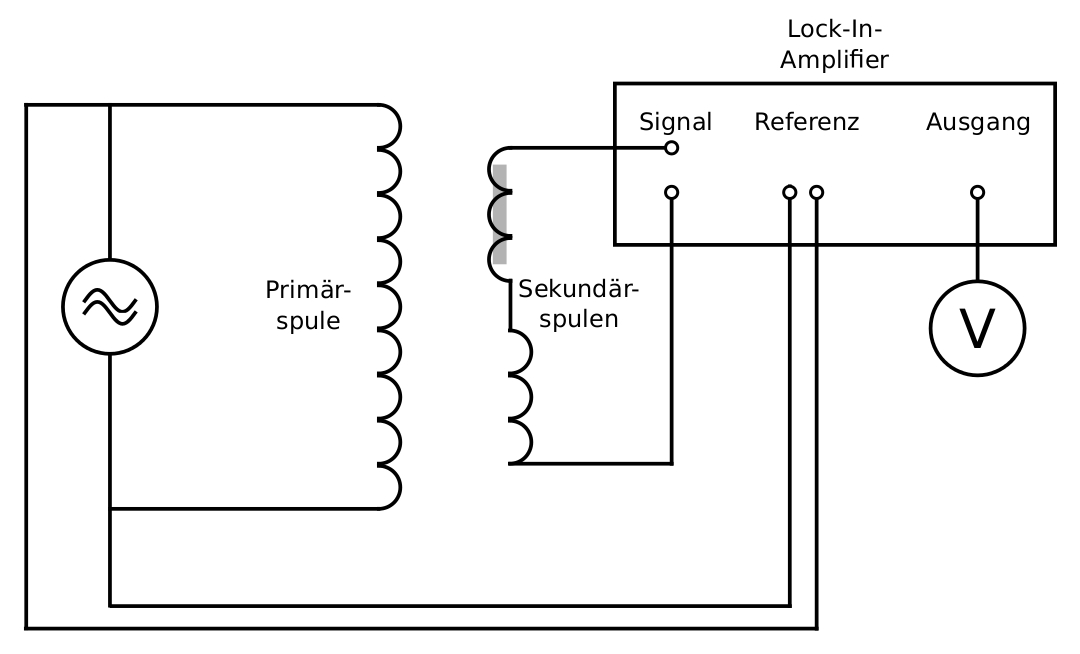
\includegraphics[width=0.7\textwidth]{data/Aufbau.jpg}
  \caption{Aufbau zur Messung der magnetischen Suszeptibilität. \cite{anleitung}}  
  \label{fig:Bild1}
\end{figure}


An der Primärspule liegt eine Referenz-Wechselspannung an, die in den astatisch gewickelten Sekundärspulen Spannungen induzieren, die sich ohne Probe im Idealfall gerade aufheben sollten. Tatsächlich tritt aber immer ein Leersignal auf, außerdme befindet sich die Probe in einer der Sekundärspulen. D.h. die gemessene Spannung besteht aus zwei Anteilen: 

$$U_{total}(T) = U_{leer} + U_{Probe}(T)$$

Sie ist proportional zur magnetischen Suszeptibilität der Probe. In einem Lock-In-Verstärker wird die Spannung $U_{total}(T)$ mittels der Referenzspannung moduliert, was in einer Gleichspannung resultiert, die wir messen. Später erfolgt eine Temperatur-Kalibration. Im oberen Teil des heliumgefüllten Dewargefäßes ist außerdem ein Druckmessgerät angeschlossen.

Zuerst muss der Kryostat befüllt werden. Nachdem das äußere Dewargefäß mit flüssigem Stickstoff befüllt worden ist, kann Helium in den Probenraum übergehoben werden. Da wir nach dem Prinzip der Verdampfungskühlung arbeiten, muss im Folgenden Helium aus dem inneren Dewargefäß in die Helium-Rückleitung abgepumpt werden, um hinreichend tiefe Temperaturen zu erreichen. Dazu steht uns eine Drehschieber-Vakuumpumpe zur Verfügung, deren Saugleistung über ein grobes und ein feines Regelventil gedrosselt werden kann. 

\section{Aufnahme der Abkühlkurve}

Zunächst nehmen wir die Spannungswerte für den Abkühlvorgang auf. Dazu öffnen wir schrittweise die Regelventile der Vakuumpumpe und senken damit den Druck und somit die Temperatur. Durch gleichzeitiges Ablesen der Spannung nehmen wir 20 Wertepaare zwischen 744 Torr und 4 Torr auf, was Temperaturen zwischen 4,2 K und 1,5 K entspricht.

\section{Aufnahme der Aufwärmkurve}

Anschließend werden die Regelventile geschlossen und die Drehschieberpumpe abgestellt. Durch die Erwärmung des Heliums erfolgt ein Druckanstieg, wobei wir wieder die Spannung ablesen und auf diese Weise 31 Wertepaare von 4 Torr bis 220 Torr aufnehmen.

\chapter{Auswertung}

\section{Druckkorrektur}

Da der Druck nicht direkt am Probenort gemessen wird, sondern an der Oberfläche des Heliumbehälters, muss die Druckdifferenz betrachtet werden, die durch das Gewicht der Heliumsäule oberhalb der Probe entsteht. Der Druck am Probenort berechnet sich wie folgt: 
$$p_{Probe} = p_{oben} + p_{He} = p_{oben} + \rho_{He} h g$$
mit der Füllhöhe h des flüssigen Heliums und dessen Dichte $\rho_{He} = 0,145 ~ \frac{g}{cm^3}$. Da am Kryostaten eine Skala angebracht ist, deren Nullpunkt am Probenort liegt, kann die Höhe direkt abgelesen werden. Beim Abkühlvorgang wurde die Höhe dreimal abgelesen und zweimal (zu Beginn und zum Ende) beim Aufwärmen. In folgender Tabelle sind die gemessenen Füllhöhen sowie die Korrekturwerte inkl. der sich dadurch ergebenden Temperaturkorrekturen aufgelistet:

\begin{center}
  \begin{tabular}{|p{1.6cm}|p{2.4cm}|p{1.6cm}|p{2cm}|p{2.4cm}|p{2cm}|p{2cm}|}
    \hline
    T in K & $p_{oben}$ in Torr & h in cm & $\Delta p$ in Torr & $p_{Probe}$ in Torr & $\Delta T$ in K & $T_{Probe}$ in K \\ \hline
    4,2 & 744 & 22,2 & 2,369 & 746,369 &  &   \\ \hline
    2,27 & 47 & 13,5 & 1,440 & 48,440 &  &    \\ \hline
    1,5 & 4 & 10,8 & 1,152 & 5,152 &  &    \\ \hline
     & 220 & 10,6 & 1,131 & 221,131 &  &    \\ \hline
	\end{tabular}
\end{center}

\section{Überprüfung des Curie- und Curie-Weiss-Gesetzes}
\begin{figure}[H]
\begin{tikzpicture}
\begin{axis}[
  default,
  title={Kalibration des sekundären Thermometers},
  xlabel=$T$ in $K$,
  ylabel=$U_{ind}$ in $mV$,
  xmin=1.4,
  xmax=4.4,
  ymin=0,
  ymax=370,
  height=0.5\linewidth
]
\addplot[
  red, only marks, mark=+, mark size=1pt, error bars/.cd, 
  y dir=both, y explicit, x dir=both, x fixed relative=0.005
] table[x index=0, y index=1, y error index=2] {data/abkuehlen.txt};
\addlegendentry{Messpunkte}
\addplot[teal, mark=x, mark size=0pt, samples=40, domain=1.4:4.4] {-151.706+753.243/x};
\addlegendentry{Curie-Fit}
\addplot[orange, mark=x, mark size=0pt, samples=40, domain=1.4:4.4] {-155.706+769.835/(0.0247+x)};
\addlegendentry{Curie-Weiss-Fit}
\end{axis}
\end{tikzpicture}
    \caption{Induzierte Spannung in Abhängigkeit der Temperatur. Die Spannung
        ist Proportional zur Magnetisierung und somit auch zur Suszeptibilität des
        Paramagneten. Sowohl der Curie als auch der Curie-Weiss fit stimmen sehr gut
        mit den gemessenen Daten überin. Lediglich an den rändern des Graphen ist
        optisch ein Unterschied der beiden Fits zu bemerken, im Bereich höherer
        Temperaturen scheint sogar der Curie-Fit eher mit den Messdaten überein zu stimmen}
\end{figure}


\subsection{Fitwerte}
Für den Curie-Fit gehen wir von einer Funktion der Form $\chi(T) \propto U_{ind}(T)
= \frac{C}{T} + U_0$ aus.
Es ergeben sich folgende Fit-Werte
\begin{center}
  \begin{tabular}{l|llll}
    \text{} & Wert     & Standardabweichung & t-Statistik & P-Wert             \\ \hline
    $C  $   & 753,243  & 5,35434            & 140,679     & $1,9388 \cdot 10^{-31}$ \\
    $U_0$   & -151,706 & 2,43924            & -62,1941    & $2,2906 \cdot 10^{-24}$ \\
  \end{tabular}
\end{center}


Für den Curie-Weiss-Fit gehen wir von einer Funktion der Form $\chi(T) \propto
U_{ind}(T) = \frac{C}{T-\theta} + U_0$ aus.
Es ergeben sich folgende Fit-Werte
\begin{center}
  \begin{tabular}{l|llll}
             & Wert       & Standardabweichung & t-Statistik & P-Wert             \\ \hline
    $C     $ & 769,835    & 44,7269            & 17,2119     & $4,7859 \cdot 10^{-13}$ \\
    $U_0   $ & -155,027   & 9,18241            & -16,8831    & $6,7582 \cdot 10^{-13}$    \\
    $\theta$ & -0,0246869 & 0,0657462          & -0,375489   & 0,711456           \\
  \end{tabular}
\end{center}
\section{Verlauf der Aufwärmung}

\section{Wärmefluss in das Helium}

\chapter{Fazit}

%ENDE INHALT
\cleardoublepage{}
% Eintrag fürs Inhaltsverzeichnis
\newpage
\begin{thebibliography}{100}
  \bibitem{anleitung} Versuchsanleitung zum Versuch Tieftemperaturmessung, heruntergeladen am 09.06.2015 von der Homepage der TU Darmstadt
  \bibitem{blackbodycoherence} The coherence length of black-body
radiation by Axel Donges, 1998: \url{http://hank.uoregon.edu/teaching-modules/Broadband-Interferometer/BBcoherence.pdf}
  \bibitem{boltzmann} Abteilung theoretische Chemie der Goethe-Universität
    Frankfurt von Prof. J. Wachtveitl: \url{http://www.theochem.uni-frankfurt.de/femtochem/lectures/PC2_Sem/Handouts-PCII-WS-12-13/Zotko_Maxwell-Boltzmann%20Verteilung.pdf}
\end{thebibliography}
\end{document}

%%% Local Variables:
%%% mode: latex
%%% TeX-master: t
%%% End:
